
\section{Identification of wave spectrum model} \label{sec:part2}

\subsection{Power Spectral Density estimate}
In this subsection we want to find the Power Spectral Density (PSD) of the wave,$\psi_w$, $S_{\psi_w}(\omega)$. To calculate the PSD the matlabfunction \textit{pwelch} was used. This function returns the Welch's PSD estimate, pxx, and a frequency vector, \cite{pwelch}.
\newline 
The following version was used $[p_{xx} , f] =  $\texttt{pwelch}($x_2$, window, noverlap, nfft, fs). The noverlap is used to overlap from segment to segment. The default of the noverlap is 50\% of the window length. Nfft is for specifies the numbers of discrete Fourier transform to use in the estimation. In the Matlab code we made the input sequence to: $psi_w(2,:)$, this to get the data from wave.mat that influence the waves have on the compass measurement. This data was given in degrees, so to get it in radians it was multiplied with pi/180  since the fs is given in radians. The sample frequency was given as 10 Hz and the window was 4096. The code used can be seen in \cref{mat:5.2.a}

\subsection{Analytic expression for transfer function and PSD}
In this subsection the task was to find an analytic expression for the transfer function of the wave response model (from $w_w$ to $\psi_w$). Ans also find an analytic expression for the Power Spectral Density function of $\psi_w$, that is $P_{\psi_w}(\omega)$.

Using the same techniques as earlier to find the transfer function from $w_w$ to $\psi_w$ using \cref{eq:xidot_def} 
\begin{equation*}
    \xi_w(s) = \frac{\psi_w(s)}{s}
\end{equation*}
with $\xi_w(0) = 0$, inserting into \cref{eq:psidot_m} and using some algebra skills, we get
\begin{equation} 
    H(s) =  \frac{\psi_{w}(s)}{w_{w}(s)} = \frac{s K_w}{s^2 + 2\lambda w_w s + \omega_0^2}
\end{equation}
Then H(s) is a stable transfer function, and the PSD for $\psi_w$ can be found though stationary analysis by using the formula under from \cite{brown12}
%Power Spectral Density of $\psi_w \rightarrow P_{\psi_w}(\omega)$. Using Fourier transform. Know that white noise have zero-mean. Random process r(t) 
\begin{equation}
\begin{split}
    P_{\psi_w}(\omega) &= |\hat{H}(j\omega)|^2 P_{\omega_w}(\omega)\\ 
    &= H(j\omega)H(-j\omega) P_{\omega_w}({\omega})
\end{split}
\end{equation}
The amplitude of $w_w$ is $P_w(j\omega)$, which is white noise, that is a constant and here is equal to 1. 
\begin{equation}
\begin{split}
    H(j\omega)H(-j\omega) &= \frac{j\omega K_w}{(j\omega)^2 + 2\lambda w_0 j\omega + \omega_0^2}*\frac{-j \omega K_w}{(-j\omega)^2 - 2\lambda w_0 j\omega + \omega_0^2} \\
    &= \frac{(\omega K_w)^2}{\omega^4 - 2\omega^2 \omega_0^2 + 4 \lambda^2 \omega_0^2 \omega^2 + \omega_0^4}
\end{split}
\end{equation} 
Thus the PSD becomes 
\begin{equation}
\begin{split}
   P_{\psi_w}(\omega)= \frac{(\omega K_w)^2}{\omega^4 - 2\omega^2 \omega_0^2 + 4 \lambda^2 \omega_0^2 \omega^2 + \omega_0^4}
\end{split}
\end{equation} 


\subsection{Resonance frequency from estimated PSD} \label{sec:5.2.c}
In this subsection the task was to find $\omega_0$, from the estimated PSD found in Power Spectral Density estimate.
\newline
\newline
The $\omega_0$ is the maximum of the power spectral density function, $S_{\psi_w}(\omega)$, and describes the frequency of waves that has the greatest impact on the head of the ship. 
\begin{figure}[H]
    \centering
    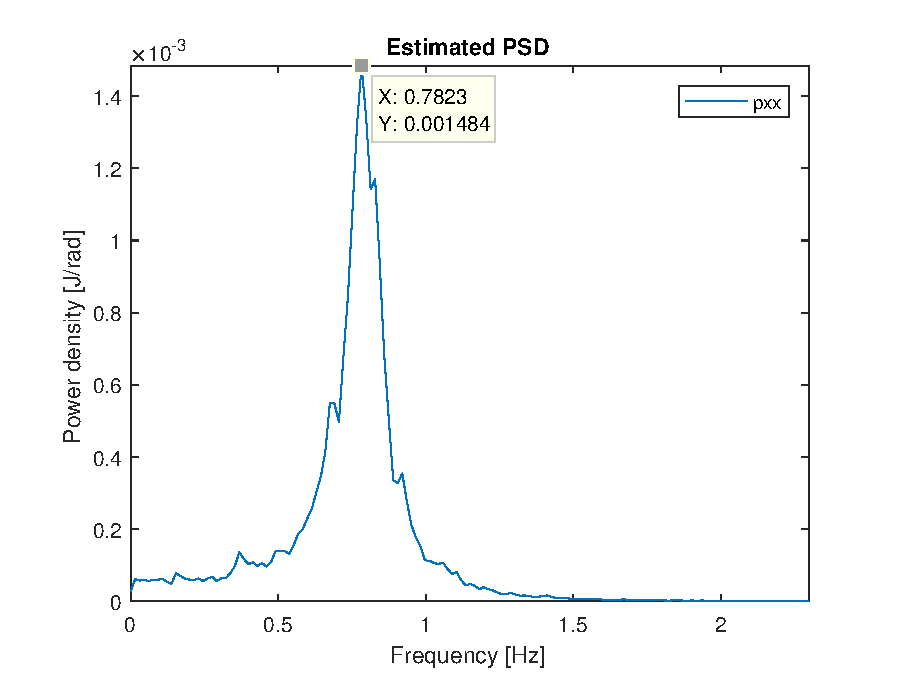
\includegraphics[width=0.8\linewidth]{Part2_pics/p2c_omega0.eps}
    \caption{Reading off $\omega_0$ from the estimated PSD found in 5.2.a}
    \label{fig:p2c}
\end{figure}
From the figure it was easy to determine that $\omega_0$ was
\begin{equation}
    \omega_0 = 0.7823
\end{equation}



\subsection{Damping factor $\lambda$} \label{sec:5.2.d}
For completing the model of the wave response, the damping factor was to be determent, $\lambda$. In the task $K_w$ was defined as $2 \lambda \omega_0 \sigma$ where $\sigma^2$ was the peak value of $P_{\psi_w}(\omega)$. To solve this task we decided to use the trial and error method. By trying different values of $\lambda$ that fitted the $P_{\psi_w}(\omega)$ to the estimate of the PSD, we have whats show in \cref{fig:p2d1} - \ref{fig:p2d2}. The final pick for $\lambda$ was 0.07. In \cref{mat:5.2.a} it is shown how the PSD function was plotted. 

\begin{figure}[H]
\begin{subfigure}{0.5\textwidth}
    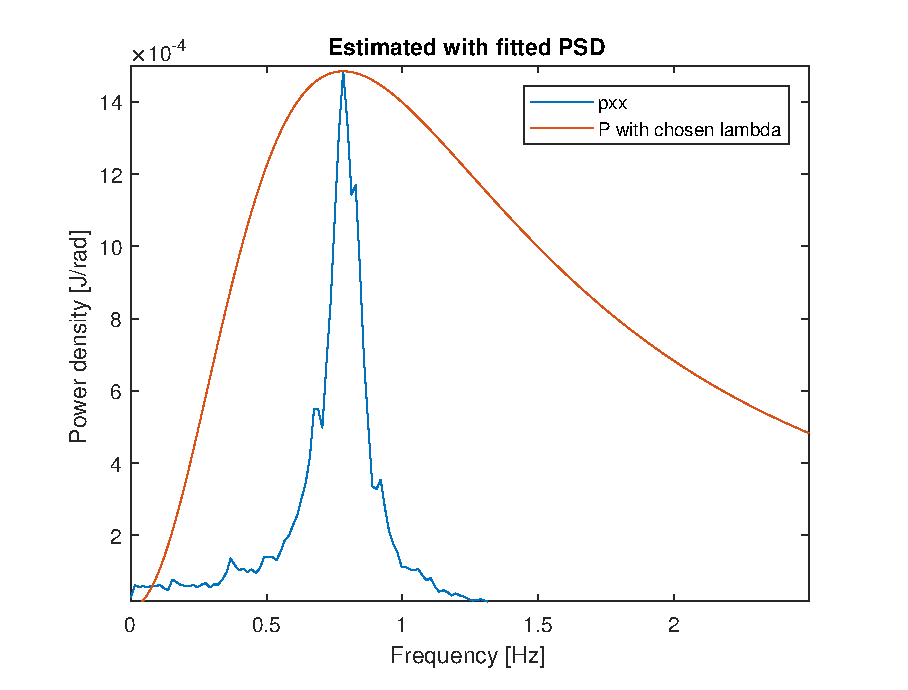
\includegraphics[width=1\linewidth]{Part2_pics/p2d_lambda_1.eps}
    \caption{$\lambda = 1$}
\end{subfigure}
\begin{subfigure}{0.5\textwidth}
    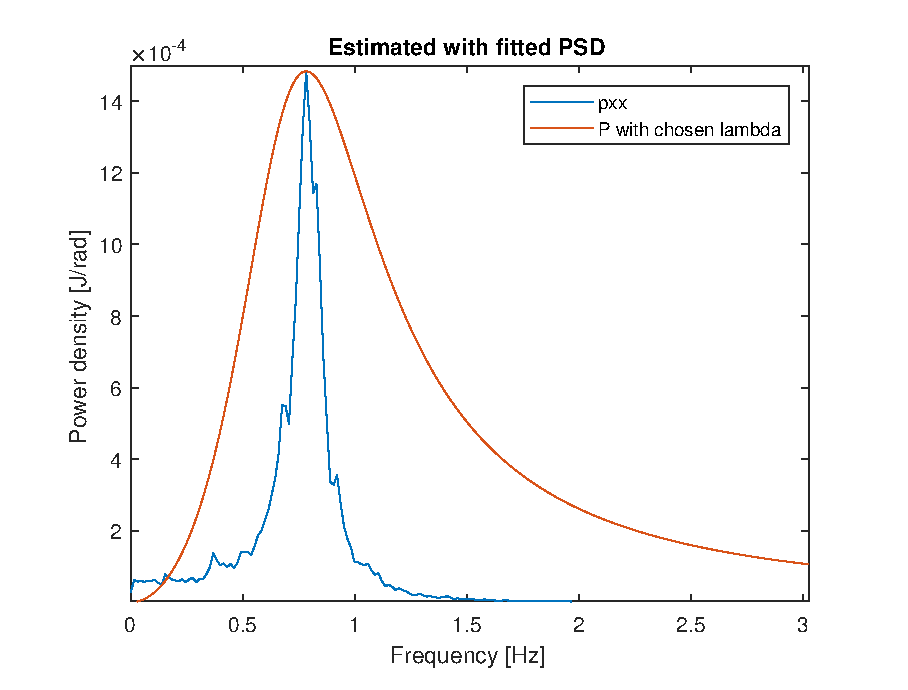
\includegraphics[width=1\linewidth]{Part2_pics/p2d_lambda_05.eps}
    \caption{$\lambda = 0.5$}
\end{subfigure}
\caption{To large values for $\lambda$}
\label{fig:p2d1}
\end{figure}

\begin{figure}[H]
\begin{subfigure}{0.5\textwidth}
    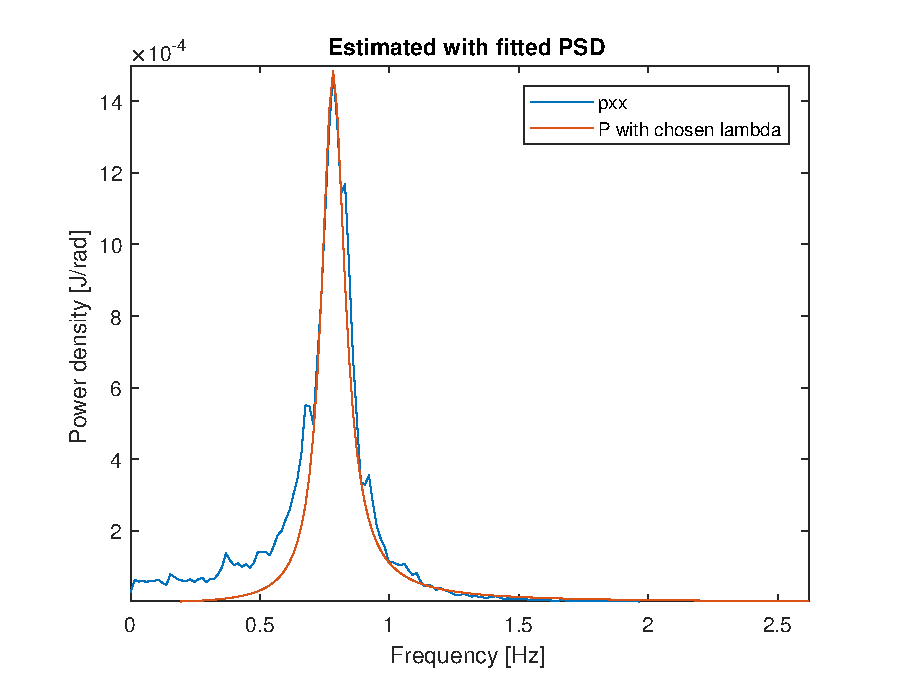
\includegraphics[width=1\linewidth]{Part2_pics/p2d_lambda_007.eps}
    \caption{$\lambda = 0.07$}
\end{subfigure}
\begin{subfigure}{0.5\textwidth}
    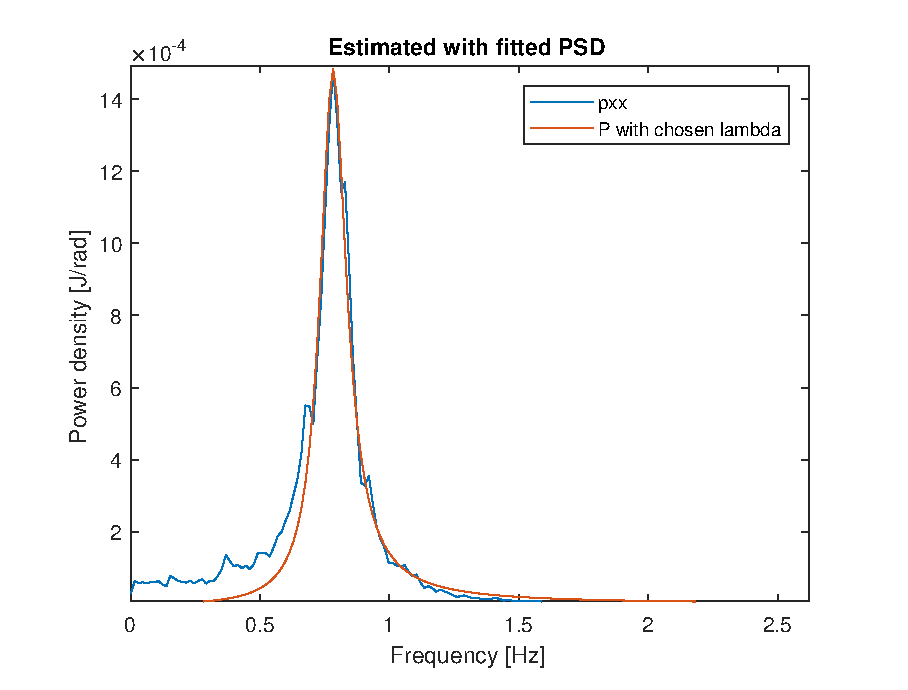
\includegraphics[width=1\linewidth]{Part2_pics/p2d_lambda_008.eps}
    \caption{$\Lambda = 0.08$}
\end{subfigure}
\caption{The best found values for $\lambda$}
\label{fig:p2d2}
\end{figure}